% Ubah judul dan label berikut sesuai dengan yang diinginkan.
\section{Metode Penelitian}
\label{sec:arsitektur}

% Ubah paragraf-paragraf pada bagian ini sesuai dengan yang diinginkan.

\begin{figure*}
  \centering
  \subfloat{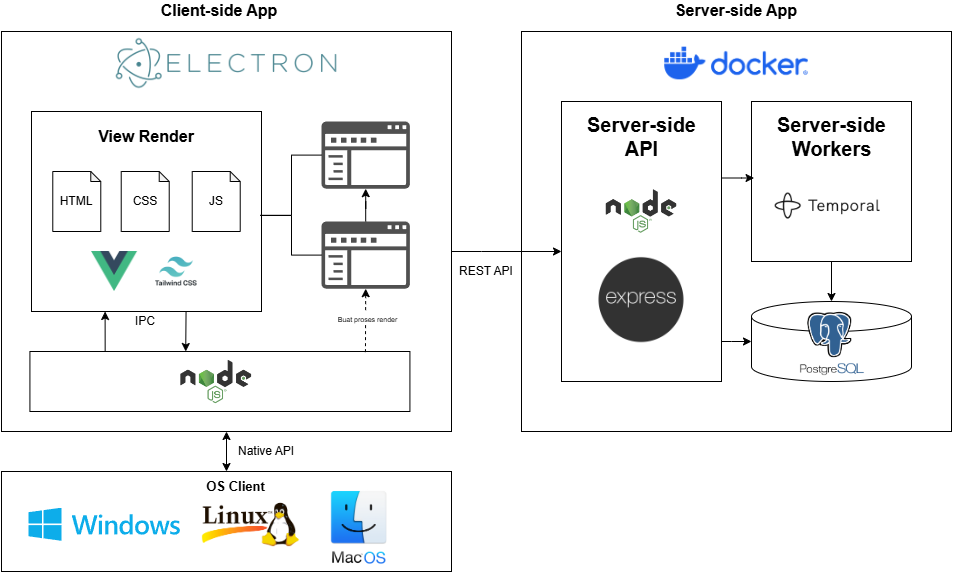
\includegraphics[width=.6\textwidth]{gambar/Arsitektur.png}}
  \hfil
  \caption{Arsitektur Sistem}
  \label{fig:structure-system}
\end{figure*}

Dalam penyelesaian tugas akhir ini, diperlukan penggunaan suatu metode tertentu yang akan menjadi dasar selama proses pengerjaan. Untuk memperkuat penggunaan metode tersebut, diperlukan serangkaian langkah yang tergambar dalam diagram alir pada \textbf{Gambar \ref{fig:flow}} berikut.

\subsection{Perumusan Masalah}
Langkah pertama dalam penelitian ini adalah mengidentifikasi perumusan masalah. Proses penentuan perumusan masalah didasarkan pada latar belakang permasalahan yang sedang dihadapi. Hasil akhir dari proses ini adalah perumusan masalah untuk menciptakan suatu sistem integrasi data dengan menggunakan metode ETL.

\subsection{Studi Literatur}
Saat melakukan studi literatur, peneliti melakukan pencarian dalam berbagai bentuk sumber seperti jurnal, buku, dan referensi lainnya untuk memberikan dukungan dalam menyelesaikan tugas akhir ini. Rentang waktu sumber referensi ini dibatasi hingga maksimal sepuluh tahun dari tahun penulisan penelitian ini. Beberapa referensi yang penting bagi penulis dalam tugas akhir ini meliputi topik integrasi data, heterogenitas data, metode ETL, serta konsep pemrograman aplikasi seperti Temporal.io, EletronJS, NextJS, Javascript, dan Basis data SQL yang mencakup PostgreSQL dan MySQL.

\subsection{Penggalian Kebutuhan}
Tahap penggalian kebutuhan melibatkan pengumpulan data tentang kebutuhan perangkat lunak integrasi data. Perangkat lunak integrasi data merupakan perangkat lunak yang dapat melakukan migrasi data dengan menggunakan metode ETL. Dalam pembangunan perangkat lunak dilakukan penggalian kebutuhan melingkupi proses bisnis, analisis kebutuhan data cabang rumah sakit, analisis kebutuhan integritas data, analisis kebutuhan fungsional, analisis resiko, dan arsitektur sistem.

\subsubsection{Proses Bisnis}
Proses bisnis perangkat lunak secara umum dapat dibagi menjadi tiga tahap. Pertama, menambahkan, melihat, mengubah, dan menghapus basis data sumber. Kedua, membuat koneksi migrasi. Ketiga, menjalankan proses migrasi dengan ETL Ketiga proses bisnis tersebut merupakan fitur utama dari perangkat lunak. Pada proses Menambahkan, melihat, mengubah, dan menghapus sumber basis data, pengguna bisa melakukan fitur tersebut pada basis data sumber yang akan di migrasi ke basis data sentra. Pada fitur menambahkan basis data sumber, pengguna harus memasukkan informasi parameter koneksi basis data. Selanjutnya sistem akan melakukan validasi terhadap informasi basis data sumber yang dimasukkan pengguna dengan cara melakukan koneksi ke basis data sumber. Jika koneksi berhasil, maka sistem akan menyimpan informasi basis data sumber yang dimasukkan pengguna ke dalam basis data perangkat lunak. 

Selanjutnya, terdapat proses membuat koneksi migrasi yang melibatkan proses pembuatan koneksi yang diperlukan untuk melakukan migrasi data dari sumber basis data ke basis data sentral. Tahapan ini memfokuskan pada konfigurasi parameter koneksi antara basis data sumber yang telah ditambahkan dan basis data sentral serta memilih tabel yang dimigrasi pada basis data sumber. Uji koneksi juga dilakukan untuk memastikan ketersediaan data yang akan dimigrasikan.

Proses terakhir adalah menjalankan proses migrasi dengan ETL. Tahapan ini terfokus pada eksekusi migrasi data dari sumber basis data baru ke dalam basis data sentral menggunakan metode ETL. Pada tahapan ini, parameter ETL disesuaikan sesuai dengan kebutuhan integrasi yang telah ditentukan sebelumnya. Setelah pemeriksaan prasyarat, proses ETL dilaksanakan dengan memanfaatkan data yang tersedia dari sumber basis data baru.

\subsubsection{Analisis Risiko}
Analisis risiko dilakukan untuk mengidentifikasi resiko yang mungkin terjadi selama proses perpindahan data. Berikut adalah resiko yang mungkin terjadi selama proses perpindahan data \citet{Hussien2021}.
\subsubsection{Koneksi basis data sumber atau sentral terputus}. 
  Risiko ini dapat terjadi karena beberapa hal seperti koneksi internet yang tidak stabil, server basis data sedang dalam perbaikan, atau server basis data sedang mengalami gangguan.  Jika koneksi basis data sumber terputus, maka sistem akan memberikan notifikasi \emph{error} kepada pengguna dan meminta pengguna untuk memperbaiki koneksi basis data. Ketika koneksi terputus saat proses migrasi, maka sistem perlu melakukan penanganan khusus untuk mengatasi hal tersebut. Strategi untuk menangani resiko ini adalah implementasi sistem yang dapat mengulangi kembali proses migrasi data.
  \subsubsection{Duplikasi data}.
  Duplikasi data adalah risiko yang terjadi apabila terdapat data yang sama pada basis data sentral. Risiko ini dapat terjadi karena beberapa hal seperti kesalahan pada proses migrasi data, kesalahan pada proses transformasi data, kesalahan pada proses penyimpanan data atau data yang sama pernah dimigrasi sebelumnya.
  \subsubsection{Kehilangan data}.
  Risiko ini dapat terjadi karena beberapa hal seperti kesalahan pada proses migrasi data, kesalahan pada proses transformasi data, atau kesalahan pada proses penyimpanan data. Penanganan risiko ini adalah dengan melakukan validasi data setelah proses migrasi. Jika terdapat data yang hilang maka sistem akan memberikan notifikasi kepada pengguna.
  \subsubsection{Ancaman keamanan data}.
  Risiko ini dapat terjadi karena beberapa hal seperti kebocoran data, peretasan sistem, atau kesalahan pada proses migrasi data. Penanganan risiko ini adalah dengan melakukan enkripsi data pada sistem dan data yang sedang dimigrasi. Selain itu, sistem juga akan melakukan validasi data setelah proses migrasi untuk memastikan bahwa data yang dimigrasi sesuai dengan data yang ada pada basis data sumber.


\subsubsection{Arsitektur Sistem}
Perangkat lunak integrasi data dibangun berbasis dekstop dengan menggunakan Eletron JS dan NextJS. Proses bisnis perangkat lunak dijalankan pada sisi \emph{backend} yang dibangun dengan arsitektur REST API menggunakan NodeJS dan ExpressJS. Pertukaran data antara \emph{backend} dan \emph{frontend} dilakukan dengan menggunakan protokol HTTP. Proses untuk melakukan migrasi data menggunakan metode ETL dijalankan pada sisi \emph{backend} dengan menggunakan Temporal.io sebagai perangkat pendukung. Dalam menjalankan migrasi ini, Temporal.io berperan penting dalam mengatur alur kerja yang kompleks, memastikan bahwa setiap tahap ekstraksi data dari sumber, transformasi data ke dalam format yang diinginkan, dan pemuatan data ke dalam sistem target dilakukan secara terkoordinasi dan efisien. Perangkat lunak ini membutuhkan basis data untuk menyimpan informasi basis data sumber dan basis data sentral. Basis data yang digunakan adalah basis data SQL dengan menggunakan PostgresSQL. \emph{Backend}, basis data aplikasi, serta Temporal.io diatur dalam lingkungan yang terisolasi menggunakan Docker Compose. Dengan Docker Compose, semua layanan ini dikemas dalam kontainer yang terpisah namun dapat saling berkomunikasi melalui jaringan internal yang dikelola oleh Docker. Konfigurasi Docker Compose memungkinkan pengembang untuk mendefinisikan dan menjalankan aplikasi multi-kontainer dengan mudah. Setiap kontainer, seperti \emph{backend}, basis data, dan Temporal.io, memiliki lingkungan eksekusi yang konsisten dan terstandarisasi, yang memastikan bahwa dependensi dan konfigurasi tetap konsisten di berbagai tahap pengembangan, pengujian, dan produksi. Arsitektur sistem perangkat lunak integrasi data dapat dilihat pada \textbf{Gambar \ref{fig:structure-system}}.

\subsection{Pembangunan Sistem}
Tahapan pembangunan sistem dilakukan secara bertahap, mengikuti urutan atau prioritas yang telah ditetapkan pada tahap penggalian kebutuhan. Selama pembangunan sistem, perhatian khusus diberikan pada keseluruhan use-case yang telah disusun sebelumnya. Pembangunan sistem ini terstruktur dalam lima komponen utama dengan rincian sebagai berikut.
  \subsubsection{Modul Koneksi}
  Komponen ini memungkinkan pengguna untuk memasukkan data sumber SQL seperti MySQL atau PostgreSQL dan menyimpannya sebagai Koneksi dalam sistem. Pada komponen ini akan disediakan antarmuka di mana pengguna dapat memasukkan detail data sumber seperti string koneksi, kredential yang meliputi username dan password. Sistem akan melakukan verifikasi pada data masukan untuk memastikan bahwa format data sesuai dengan jenis sumber data yang dimasukkan, sebagai contoh user wajib menuliskan user dan password apabila pengguna ingin memasukkan basis data MySQL sebagai \emph{"Source"} tersebut. Setelah itu sistem menyimpan hasil masukkan pengguna ke dalam basis data lokal yang tergabung pada sistem.

  \subsubsection{Pembuatan Koneksi Migrasi}
  Komponen ini memungkinkan pengguna untuk membuat koneksi migrasi antara sumber basis data dan tujuan basis data. Basis data tujuan atau \emph{"Destination"} merupakan basis data central yang menjadi tujuan integrasi data ini. Pada proses pembuatan koneksi, pengguna diharuskan memilih tabel yang akan dimigrasi dari basis data sumber ke basis data tujuan. Sistem akan melakukan ekstrasi metadata pada tabel yang dipilih guna mendapatkan informasi kolom tabel. Informasi koneksi yang mancakup id \emph{"Source"}, tabel yang dipilih, serta informasi tambahan lain disimpan dalam basis data perangkat lunak.

  \subsubsection{Modul Pekerjaan Migrasi Data}
  Komponen ini merupakan bagian utama dari aplikasi, yaitu proses ETL yang melibatkan proses perpindahan data dari sumber ke basis data tujuan. Tahapan migrasi mencakup tiga aktivitas, yaitu:
    \begin{enumerate}
      \item Ekstraksi data, pada tahap ini dilakukan pembacaan data dari basis data sumber dan tabel-tabel yang dipilih. Proses ini melibatkan pengambilan data menggunakan metode yang sesuai dengan sumber data yang digunakan.

      \item Transformasi data, setelah data diekstraksi, dilakukan proses transformasi di mana data yang telah diekstrak dimodifikasi, diformat ulang, atau diperkaya dengan informasi tambahan sesuai kebutuhan. Contoh proses transformasi adalah penambahan kolom-kolom baru, pengubahan format data, atau penggabungan data dari beberapa sumber.

      \item Muat data, pada tahap ini data yang telah melalui proses transformasi dimuat ke dalam basis data tujuan. Proses ini melibatkan penyimpanan data ke dalam struktur basis data yang sesuai dengan menggunakan koneksi yang tersedia untuk berbagai jenis basis data seperti MySQL dan PostgreSQL
    \end{enumerate}
  
    \subsubsection{Modul Authentifikasi}
    Komponen ini bertanggung jawab untuk memastikan keamanan data pada keseluruhan perangkat lunak integrasi data. Komponen ini terdiri dari tiga sub-komponen, yaitu:
    \begin{enumerate}
      \item Authentifikasi, komponen ini mengatur hak akses pada perangkat lunak dengan menerapkan sistem login. Sistem login ini memungkinkan pengguna untuk mengakses perangkat lunak dengan menggunakan username dan password yang telah didaftarkan sebelumnya. Komponen ini memastikan bahwa hanya pengguna yang memiliki hak akses yang dapat mengakses perangkat lunak.
    \end{enumerate}


\subsection{Pengujian Sistem}
Tahap pengujian sistem merupakan langkah penting yang dilakukan oleh penulis untuk memeriksa fungsi dari sistem integrasi yang sedang dikembangkan. Tahap pengujian ini sebaiknya dilakukan bersamaan dengan proses pengembangan guna memastikan bahwa sistem informasi beroperasi sesuai yang diharapkan.

\subsubsection{\emph{Fungsional Testing}}
Pengujian fungsional digunakan untuk mengevaluasi kehandalan sistem yang telah dibuat berdasarkan skenario use-case yang telah ditetapkan sebelumnya. Tujuan dari pengujian ini adalah memastikan bahwa setiap fitur berjalan dengan baik dan sesuai fungsinya dalam sistem. Selain itu, pengujian ini juga memverifikasi kinerja fitur-fitur tersebut dengan melakukan pengawasan pada proses internal sistem. Pengujian dilakuakan dengan metode \emph{white-box testing} dengan cara melihat \emph{source code} yang ada pada sistem dan menentukan fungsi pada \emph{use case} untuk memeriksa sebuah kondisi telah dieksekusi dengan tepat sehingga menghasilkan keluaran yang valid. Teknik yang akan digunakan dalam pengujian white box ini adalah \emph{statement coverage}. Pengujian unit dapat dikatakan berhasil jika nilai \emph{statement coverage} mencapai 100\%. Jika hasil yang diperoleh sesuai dengan yang diharapkan, maka fitur tersebut dinyatakan berhasil. Namun jika hasil yang diperoleh tidak sesuai dengan yang diharapkan, maka fitur tersebut dinyatakan gagal dan perlu dilakukan perbaikan.

\subsubsection{Uji Kualitas Data Migrasi}
Pengujian kualitas data digunakan untuk mengevaluasi data hasil migrasi guna memastikan bahwa data yang dipindahkan dari sistem lama ke sistem baru tetap akurat, lengkap, dan konsisten. Proses pengujian ini melibatkan beberapa langkah penting. Pertama, dilakukan pengecekan integritas data untuk memastikan bahwa semua data yang telah dimigrasikan tidak mengalami kerusakan atau kehilangan selama proses migrasi. Langkah ini mencakup verifikasi checksum, penghitungan total baris, dan validasi struktur data. Kedua, dilakukan pengujian konsistensi data untuk memastikan bahwa data yang dimigrasikan tetap konsisten dan sesuai dengan aturan bisnis yang telah ditetapkan. Ini termasuk memeriksa referensi silang antar tabel, validasi nilai-nilai unik, dan memastikan tidak ada duplikasi data yang tidak diinginkan. Langkah-langkah ini memastikan bahwa data yang telah dimigrasikan ke sistem baru dapat diandalkan dan siap digunakan tanpa masalah lebih lanjut. Hasil pengujian kualitas data disajikan dalam bentuk tabel untuk mempermudah analisis dan identifikasi area yang memerlukan perhatian lebih lanjut.

\begin{figure} [ht]
  \centering
  % Ubah sesuai dengan nama file gambar dan ukuran yang akan digunakan.
  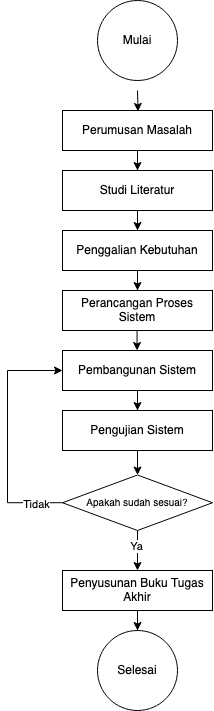
\includegraphics[width=0.1\textwidth]{gambar/flow_fix5.png}

  % Ubah sesuai dengan keterangan gambar yang diinginkan.
  \caption{Diagram alir penelitian}
  \label{fig:flow}
\end{figure}


% \begin{figure} [ht]
%   \centering
%   % Nama dari file gambar yang diinputkan
%   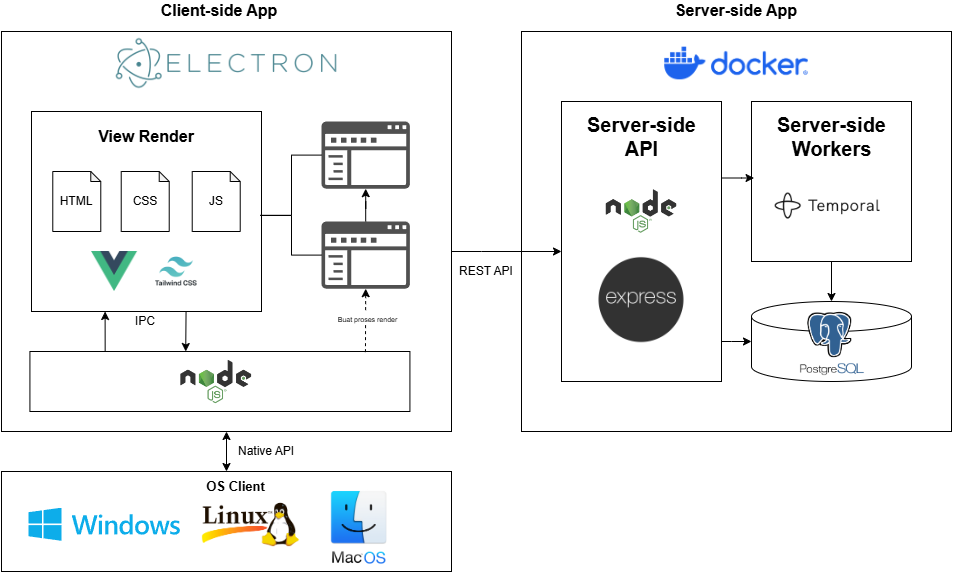
\includegraphics[width=0.4\textwidth]{gambar/Arsitektur.png}
%   % Keterangan gambar yang diinputkan
%   \caption{Diagram struktur sistem}
%   % Label referensi dari gambar yang diinputkan
%   \label{fig:structure-system}
% \end{figure}

% \subsection{Cetak Biru Roket}
% \label{subsec:cetakbiruroket}

% Pada cetak biru yang tertera pada Gambar \ref{fig:cetakbiru}. \lipsum[8]

% % Contoh input gambar pada kolom.
% \begin{figure} [ht]
%   \centering
%   % Ubah sesuai dengan nama file gambar dan ukuran yang akan digunakan.
%   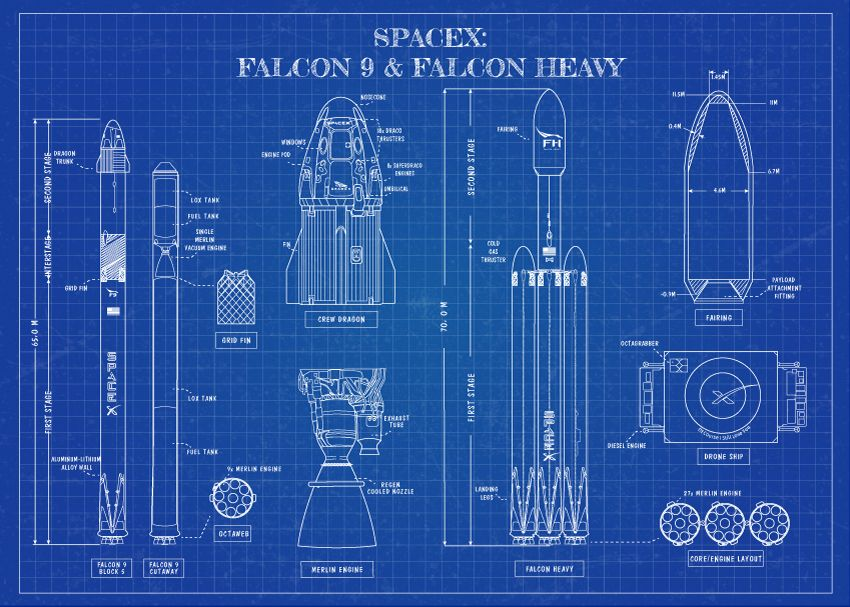
\includegraphics[width=0.4\textwidth]{gambar/cetakbiru.jpg}

%   % Ubah sesuai dengan keterangan gambar yang diinginkan.
%   \caption{Cetak biru roket yang akan diuji coba. \cite{cetakbiruspacex}}
%   \label{fig:cetakbiru}
% \end{figure}

% \lipsum[9-10]

% \subsection{Lorem Ipsum}
% \label{subsec:loremipsum}

% \lipsum[11]

% % Contoh pembuatan tabel.
% \begin{table}
%   \caption{Contoh tabel sederhana}
%   \label{tab:tabelsederhana}
%   \centering
%   \begin{tabular}{lll}
%     \toprule
%     Heading1 & Heading2 & Heading3  \\
%     \midrule
%     One      & Two      & Three     \\
%     Four     & Five     & Six       \\
%     \bottomrule
%   \end{tabular}
% \end{table}

% % Contoh pembuatan potongan kode.
% \begin{lstlisting}[
%   language=C++,
%   caption={Program halo dunia.},
%   label={lst:halodunia}
% ]
% #include <iostream>

% int main() {
%     std::cout << "Halo Dunia!";
%     return 0;
% }
% \end{lstlisting}

% \lipsum[12]

% % Contoh pembuatan daftar.
% \begin{enumerate}
%   \item \lipsum[13][1-4]
%   \item \lipsum[13][5-8]
%   \item \lipsum[13][9-12]
% \end{enumerate}

% \lipsum[14-15]
